\documentclass[tikz,border=2pt]{standalone}
\usepackage{amsmath,amssymb}
\usepackage{xcolor}
\usetikzlibrary{positioning}
\begin{document}
% Extracted from namuenofull.inc; source column: \footnotesize \cite{NU}$_{\rm p{ 161 }}$ I$^*_{0}$-II$^*$-$\alpha$
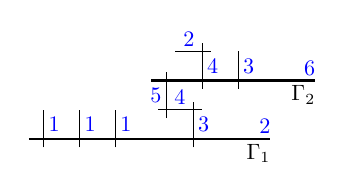
\begin{tikzpicture}[xscale=0.57,yscale=0.62]
\draw[thick,shorten >=2] (-1/3,0)--(31/6,0) node[inner sep=2pt,blue,above left,scale=0.8] {2} node[inner sep=2pt,below left,scale=0.8] {$\Gamma_1$};
\draw[shorten <=-3pt] (0,0)--node[inner sep=2pt,scale=0.8,blue,right] {1} (0,3/5);
\draw[shorten <=-3pt] (4/5,0)--node[inner sep=2pt,scale=0.8,blue,right] {1} (4/5,3/5);
\draw[shorten <=-3pt] (8/5,0)--node[inner sep=2pt,scale=0.8,blue,right] {1} (8/5,3/5);
\draw[shorten <=-3pt, shorten >=-3pt] (10/3,0)--node[inner sep=2pt,scale=0.8,blue,right] {3} (10/3,3/5);
\draw[shorten <=-3pt, shorten >=-3pt] (10/3,3/5)--node[inner sep=2pt,scale=0.8,blue,above] {4} (41/15,3/5);
\draw[shorten <=-3pt, shorten >=-3pt] (41/15,3/5)--node[inner sep=2pt,scale=0.8,blue,left] {5} (41/15,6/5);
\draw[thick,shorten >=2] (12/5,6/5)--(37/6,6/5) node[inner sep=2pt,blue,above left,scale=0.8] {6} node[inner sep=2pt,below left,scale=0.8] {$\Gamma_2$};
\draw[shorten <=-3pt, shorten >=-3pt] (53/15,6/5)--node[inner sep=2pt,scale=0.8,blue,right] {4} (53/15,9/5);
\draw[shorten <=-3pt] (53/15,9/5)--node[inner sep=2pt,scale=0.8,blue,above] {2} (44/15,9/5);
\draw[shorten <=-3pt] (13/3,6/5)--node[inner sep=2pt,scale=0.8,blue,right] {3} (13/3,9/5);
\end{tikzpicture}
\end{document}
